\subsection{\texttt{Temoa}: Business As Usual}
\begin{frame}
  \frametitle{BAU: Grid Model}
  \begin{figure}
    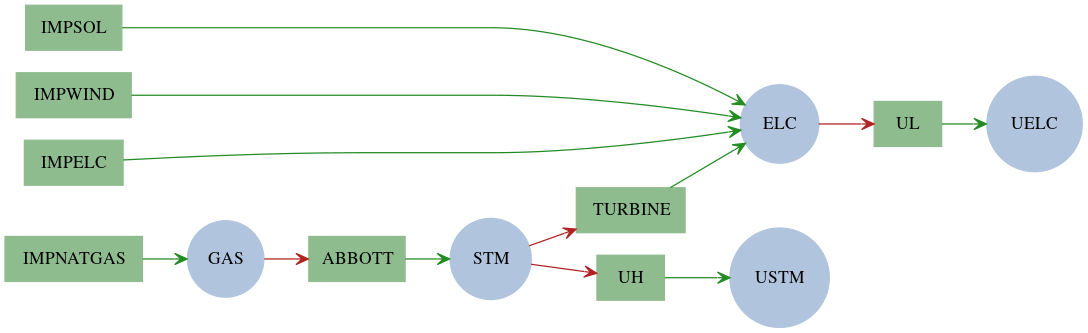
\includegraphics[width=\textwidth]{bau_temoa_uiuc.png}
    \caption{Graph representation of the UIUC embedded grid.}
    \label{fig:uiucgrid}
  \end{figure}
\end{frame}

\begin{frame}
  \frametitle{BAU: Generation}
      \begin{figure}
        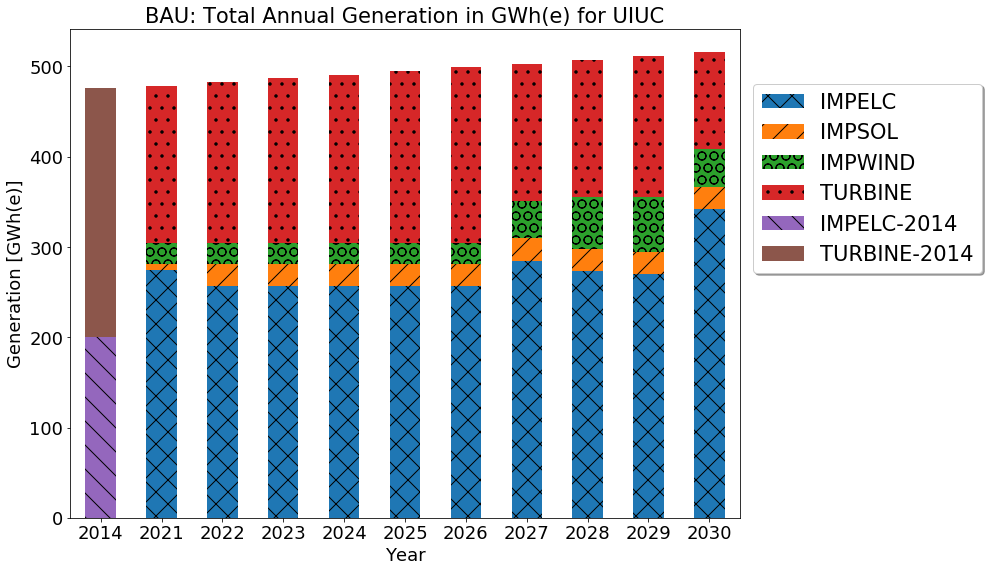
\includegraphics[width=0.8\textwidth]{bau_generation_w2014.png}
        \caption{The change in activity from each energy source from 2020-2030. Assuming 1\% demand growth each year}
        \label{fig:bau_generation}
      \end{figure}

\end{frame}

\begin{frame}
  \frametitle{BAU: Emissions}
  \begin{columns}
    \column[t]{5cm}
      \begin{figure}
        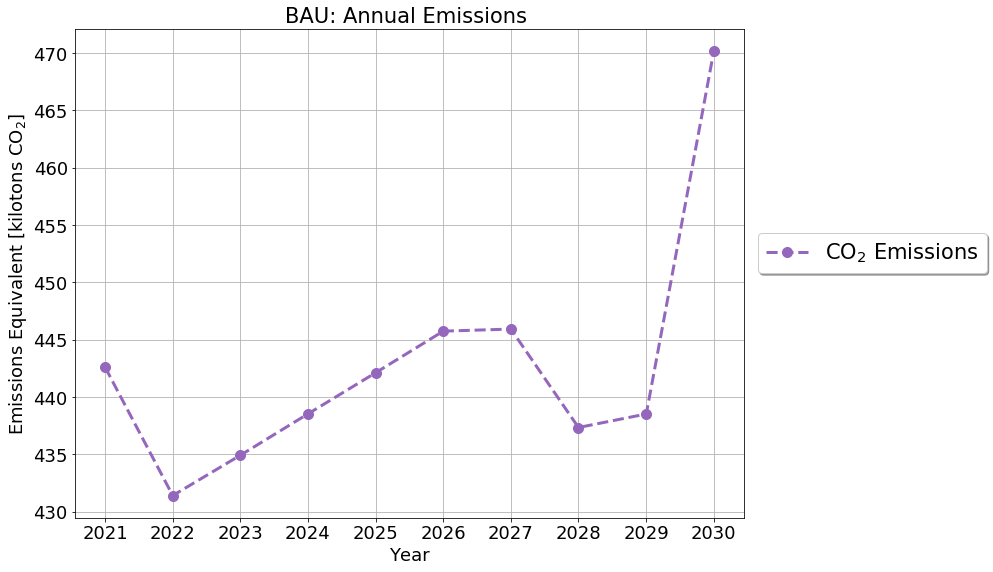
\includegraphics[width=\textwidth]{bau_emissions.png}
        \caption{The change in activity from each energy source from 2020-2030. Assuming 1\% demand growth each year}
        \label{fig:bau_generation}
      \end{figure}
    \column[t]{5cm}
    \begin{figure}
        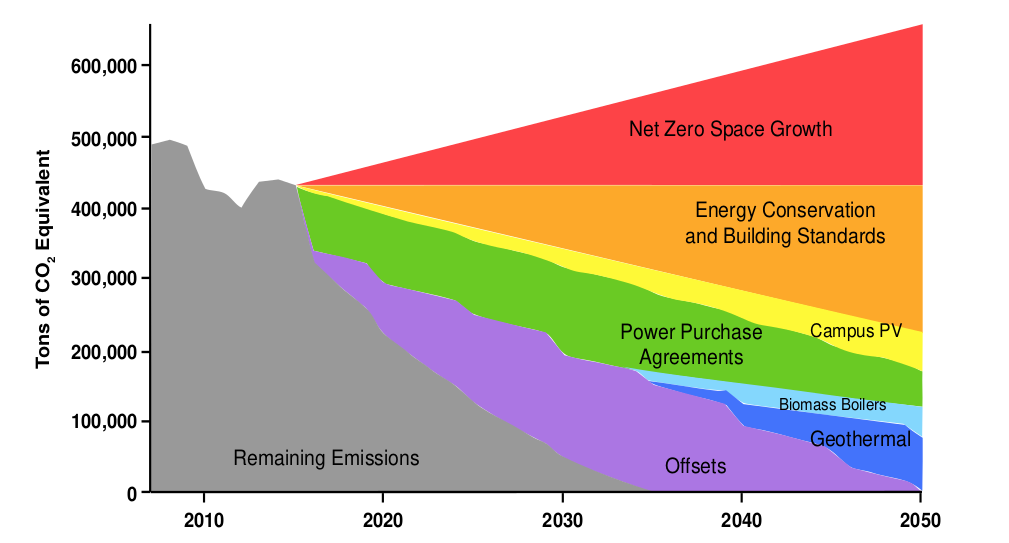
\includegraphics[width=\textwidth]{icap_uiucemissions.png}
        \caption{Predicted growth in emissions from iCAP \cite{isee_illinois_2015}.}
        \label{fig:uiuc_emissions}
      \end{figure}
  \end{columns}
\end{frame}

\subsection{\texttt{Temoa}: UIUC With Carbon Limits}
